%%
% This is an Overleaf template for presentations
% using the TUM Corporate Desing https://www.tum.de/cd
%
% For further details on how to use the template, take a look at our
% GitLab repository and browse through our test documents
% https://gitlab.lrz.de/latex4ei/tum-templates.
%
% The tumbeamer class is based on the beamer class.
% If you need further customization please consult the beamer class guide
% https://ctan.org/pkg/beamer.
% Additional class options are passed down to the base class.
%
% If you encounter any bugs or undesired behaviour, please raise an issue
% in our GitLab repository
% https://gitlab.lrz.de/latex4ei/tum-templates/issues
% and provide a description and minimal working example of your problem.
%%

\documentclass[
  german,            % define the document language (english, german)
  aspectratio=169,    % define the aspect ratio (169, 43)
  % handout=2on1,       % create handout with multiple slides (2on1, 4on1)
  % partpage=false,     % insert page at beginning of parts (true, false)
  % sectionpage=true,   % insert page at beginning of sections (true, false)
]{tumbeamer}


% load additional packages
\usepackage{booktabs}
\usepackage{graphicx}
\usepackage{tikz}
\usepackage{url}
\usepackage{pgfplots}
\usepackage{hyperref}
\usepackage{pmboxdraw}
\usepackage{float}
\usepackage{babel}[ngerman]
\usepackage{csquotes}[autostyle]
\usepackage[useregional]{datetime2}
\usepackage{listings}
\usepackage{xurl}
\usetikzlibrary{patterns}

% tikz
\usetikzlibrary{overlay-beamer-styles}
\usetikzlibrary{arrows.meta,backgrounds,positioning,shapes.symbols,decorations.pathreplacing,patterns,patterns.meta,tikzmark,chains,matrix,arrows,shapes.geometric}


\lstset {
    frame=single,
    tabsize=4,
    breaklines=true,
    xleftmargin=5pt,
    xrightmargin=5pt,
    basicstyle=\ttfamily\footnotesize,
    %language=[RISC-V]Assembler,
}

\hypersetup { 
  colorlinks=true,
  urlcolor=blue,
  filecolor=black,
  linkcolor=black
}

% tikz  
\usetikzlibrary{fit}

% image path
\graphicspath{ {../resources/} }

% presentation metadata
\title{Übung 05: Caches}
\subtitle{Einführung in die Rechnerarchitektur}
\author{\theAuthorName}

\institute{\theGroupName\\\theSchoolName\\\theUniversityName}
\date{18. -- \DTMdisplaydate{2024}{11}{24}{-1}}

\footline{\insertauthor~|~\insertshorttitle~|~\insertshortdate}


% macro to configure the style of the presentation
\TUMbeamersetup{
  title page = TUM tower,         % style of the title page
  part page = TUM toc,            % style of part pages
  section page = TUM toc,         % style of section pages
  content page = TUM more space,  % style of normal content pages
  tower scale = 1.0,              % scaling factor of TUM tower (if used)
  headline = TUM threeliner,      % which variation of headline to use
  footline = TUM default,         % which variation of footline to use
  % configure on which pages headlines and footlines should be printed
  headline on = {title page},
  footline on = {every page, title page=false},
}


% available frame styles for title page, part page, and section page:
% TUM default, TUM tower, TUM centered,
% TUM blue default, TUM blue tower, TUM blue centered,
% TUM shaded default, TUM shaded tower, TUM shaded centered,
% TUM flags
%
% additional frame styles for part page and section page:
% TUM toc
%
% available frame styles for content pages:
% TUM default, TUM more space
%
% available headline options:
% TUM empty, TUM oneliner, TUM twoliner, TUM threeliner, TUM logothreeliner
%
% available footline options:
% TUM empty, TUM default, TUM infoline


\begin{document}

\maketitle

\begin{frame}[c]{Mitschriften \& Infos}{}
  \begin{minipage}[t]{\textwidth}
    \begin{columns}[c]
      \begin{column}{0.8\textwidth}
        Montags: \href{\zulipMo}{\zulipMo}
      \end{column}
      \begin{column}{0.2\textwidth}
        \includegraphics[width=0.8\linewidth]{\zulipMoQrFilename}
      \end{column}
    \end{columns}
  \end{minipage}
  \rule{\textwidth}{0.4pt}
  \begin{minipage}[t]{\textwidth}
    \begin{columns}[c]
      \begin{column}{0.8\textwidth}
        Donnerstags: \href{\zulipDo}{\zulipDo}
      \end{column}
      \begin{column}{0.2\textwidth}
        \includegraphics[width=0.8\linewidth]{\zulipDoQrFilename}
      \end{column}
    \end{columns}
  \end{minipage}
  \ifdefined\myWebsite
  \rule{\textwidth}{0.4pt}
  \centering
  Website: \href{\myWebsite}{\myWebsite}
  \fi
\end{frame}

\begin{frame}[c]{}{}
  \begin{center}
    \LARGE  Keine Garantie für die Richtigkeit der Tutorfolien.

    \Large Bei Unklarheiten/Unstimmigkeiten haben VL/ZÜ-Folien recht!
  \end{center}
\end{frame}

\begin{frame}[c]{Inhaltsübersicht}{}
  \begin{columns}[c]
    \begin{column}{1\textwidth}
      \begin{itemize}
        \item Wiederholung
        \item Tutorblatt
        \begin{itemize}
          \item Speicherzugriffszeit
          \item Vergleich der Cachearten
          \item Cachestruktur und Cachemisses
          \item Ersetzungsstategien
        \end{itemize}
      \end{itemize}
    \end{column}
  \end{columns}
\end{frame}

\begin{frame}[fragile, c]{Motivation Caches}{}
  \begin{itemize}
    \item Zugriffe auf Hauptspeicher ($\equiv$ RAM) sind \textbf{extrem} langsam. Lösung: Caches
    \item \enquote{Zwischenstation} zwischen Registern (sehr schnell, sehr klein) und Hauptspeicher (sehr langsam, sehr groß)
    \item Idee: Häufig genutzte Daten im Cache zwischenspeichern, der Rest wird bei Bedarf aus dem Hauptspeicher geholt
    \item heutzutage meist L1/L2/L3-Caches: Caches aufsteigender Größe, aber absteigender Zugriffszeit
  \end{itemize}
  \centering{
    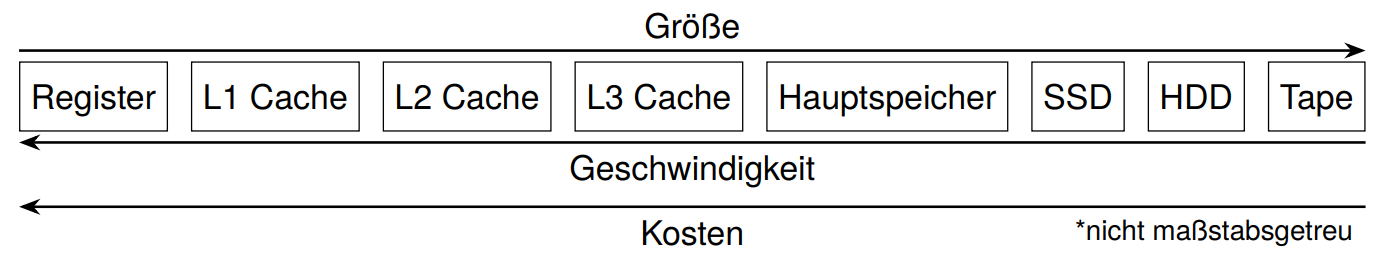
\includegraphics[width=0.9\linewidth]{w05_caches_sizes_cost_zue.png}
  }
  
\end{frame}

\newcommand{\terminologyFrame}[2]{
        \begin{frame}
            \frametitle{Cache-Terminologie}
            #1
            
            \centering
            \begin{tikzpicture}[start chain, node distance=3cm]
                \node[label=above:CPU, draw, minimum width=2cm, minimum height=2cm, on chain] (cpu) {};
                \node[label=above:Cache, draw, minimum width=2cm, minimum height=3cm, on chain] (cache) {};
                \node[label=above:Hauptspeicher, draw, minimum width=2cm, minimum height=4.5cm, on chain] (mem) {};
                
                #2
                
            \end{tikzpicture}
        \end{frame}
    }
    
    \newcommand{\arrowPair}[3][0.5cm]{
        \draw[-Stealth, very thick] ([yshift=#1]#2.east) -- ([yshift=#1]#3.west);
        \draw[-Stealth, very thick] ([yshift=-1*#1]#3.west) -- ([yshift=-1*#1]#2.east);
    }
    
    \terminologyFrame{
        \textbf{Hit Latency:} Antwortzeit, wenn Wert im Cache
    }{
        \arrowPair{cpu}{cache}
        \node[] at (cache.center) {\Huge\checkmark};
    }
    
    \terminologyFrame{
        \textbf{Miss Latency:} Antwortzeit, wenn Wert nicht im Cache
    }{
        \arrowPair{cpu}{cache}
        \arrowPair{cache}{mem}
        \node[] at (cache.center) {\Huge$\times$};
        \node[] at (mem.center) {\Huge\checkmark};
    }
    
    \terminologyFrame{
        \textbf{Miss Penalty:} Miss Latency $-$ Hit Latency
    }{
        \arrowPair{cache}{mem}
        \node[] at (mem.center) {\Huge\checkmark};
    }

\begin{frame}[c, fragile]{Terminologie}
  \begin{itemize}
    \item \textbf{Hit}: Datum liegt im Cache
    \item \textbf{Miss}: Datum nicht im Cache, muss erst aus Hauptspeicher geholt werden
    \item Ziel: möglichst hohe \textbf{Hitrate} (Hits/Anfragen) $\rightarrow$ häufig genutzte Daten im Cache
    \item \textbf{zeitliche Lokalität}: Zugriff auf x $\rightarrow$ wschl. Zugriff auf x in Zukunft
    \item \textbf{räumliche Lokalität}: Zugriff auf x $\rightarrow$ Zugriff auf Daten in der Nähe (oft durch Cacheline abgedeckt)
  \end{itemize}
\end{frame}

\begin{frame}
  \frametitle{Messung der Cache-Güte}
  \vfill
  \begin{equation*}
    \text{CPU Time} = \text{IC} \cdot \left(\dfrac{\text{CPI}}{f} + \frac{\text{Memory Accesses}}{\text{Instruction}} \cdot \text{Average Memory Access Time}\right)
  \end{equation*}
  \begin{equation*}
    \text{Average Memory Access Time} = \text{Hit Rate} \cdot \text{Hit Latency} + \text{Miss Rate} \cdot \text{Miss Latency}
  \end{equation*}
  \vfill
  {\renewcommand{\arraystretch}{1.4}
      \begin{tabular}{rl}
          Frequenz ($f$): & Frequenz des Prozessors\footnote{für uns in der Einheit $\frac{\text{cycles}}{\text{s}}$}\\
          Instruction Count (IC): & Anzahl an auszuführenden Instruktionen\\
          Cycles per Instruction (CPI): & (Durchschnitts-) Anzahl an Zyklen pro Instruktion\\
          Memory Access Rate: & (Durchschnitts-) Anzahl an Speicherzugriffen pro Instruktion\\
  \end{tabular}}
\end{frame}

\begin{frame}[c]{Aufbau eines Caches}{}
  \begin{columns}[c]
    \begin{column}{0.5\textwidth}
      \begin{itemize}
        \item Menge an Speicherzeilen einer festen Länge (Cachezeilenlänge) 
        \item Jede Speicherzeile ist mit dem Tag, einem Teil der Adresse identifiziert
        \item In einer Cachezeile steht immer ein Block an Daten, die an fortlaufenden Adressen im Speicher stehen
      \end{itemize}
    \end{column}
    \begin{column}{0.5\textwidth}
      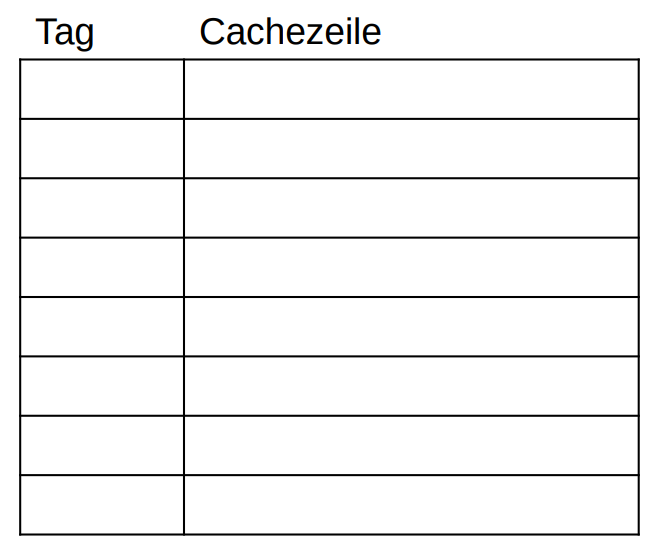
\includegraphics[width=\linewidth]{w05_aufbauchaches_rep.png}
    \end{column}
  \end{columns}
\end{frame}

\begin{frame}{Adressierung}
  \begin{itemize}
      \item 4-fach-assoziativer Cache
      \item Cachegröße: 128 Byte
      \item Cachezeile: 4 Byte
  \end{itemize}
  \vspace{-1ex}
  \begin{center}
\resizebox{.7\textwidth}{!}{
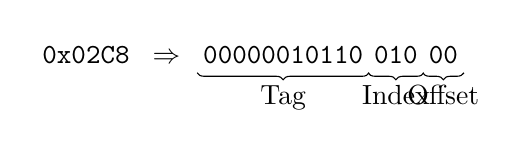
\begin{tikzpicture}[ampersand replacement=\&]
  \matrix (cache) [matrix of nodes, nodes={minimum height=1em, inner xsep=2pt, font={\ttfamily}}]
  {
    0x02C8 \&[1ex] \(\Rightarrow\) \&[1ex] 00000010110 \& 010 \& 00 \&[1ex] \\
  };
  \draw<2> [decorate, decoration = {brace, mirror}] (cache-1-5.south west) -- node[below,midway,inner ysep=1ex]{Offset} (cache-1-5.south east);
  \draw<3> [decorate, decoration = {brace, mirror}] (cache-1-4.south west) -- node[below,midway,inner ysep=1ex]{Index} (cache-1-4.south east);
  \draw<4> [decorate, decoration = {brace, mirror}] (cache-1-3.south west) -- node[below,midway,inner ysep=1ex]{Tag} (cache-1-3.south east);
\end{tikzpicture}
}
\end{center}
\vspace{-1ex}
\only<2>{\textbf{Offset Bits} -- bezeichnen das Byte der Cachezeile, auf das zugegriffen werden soll. \\Die Cachezeilengröße ist in unserem Beispiel 4 Bytes, deswegen genügen $\log_2{4}=2$ Bits.}

\only<3>{\textbf{Index Bits} -- bestimmen das Cache-Set, in dem die gewählte Adresse sein kann. \\In unserem Beispiel ist der Cache 128 Byte groß, hat eine Cachezeilen-Größe von 4 Byte und ist 4-fach-assoziativ. Also es gibt $\frac{\frac{128}{4}}{4} = 8$ Sets. Daher benötigt man hier $\lceil\log_2{8}\rceil = 3$ Bits. Die Daten werden also in Set \#2 landen.}

\only<4>{\textbf{Tag Bits} -- restliche Bits. Identifizieren die in einer Cachezeile gespeicherten Daten eindeutig.}
\end{frame}

\begin{frame}[c]{Cachearten: Direct Mapped Cache}{}
  \begin{columns}[c]
    \begin{column}{0.5\textwidth}
      \begin{itemize}
        \item Ein Datum kann auf eine Cachezeile gemapped werden 
        \item Wenn schon etwas drin steht, wird es verdrängt $\rightarrow$ möglicherweise sehr viele Verdrängungen
        \item Sehr schnelle Zugriffe $\rightarrow$ nur ein Tag vergleich notwendig
      \end{itemize}
    \end{column}
    \begin{column}{0.5\textwidth}
      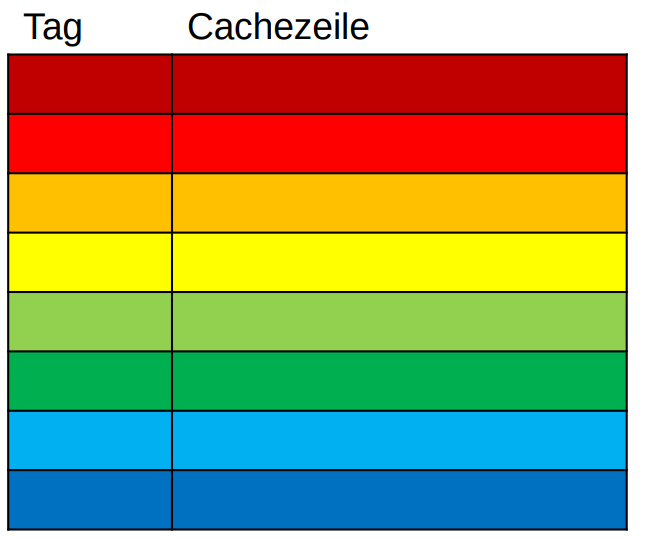
\includegraphics[width=\linewidth]{w05_directmapped_rep.png}
    \end{column}
  \end{columns}
\end{frame}

\begin{frame}[c]{Cachearten: Vollassoziativer Cache}{}
  \begin{columns}[c]
    \begin{column}{0.5\textwidth}
      \begin{itemize}
        \item Ein Datum hat keine feste Position im Cache, also keine Index Bits $\rightarrow$ wenn der Cache leer ist, laden wir einfach nacheinander die Daten in den Cache
        \item In jeder der Zeilen könnte das Datum stehen, auf das wir zugreifen wollen
        \begin{itemize}
          \item Wir müssen bei jedem Zugriff schauen ob der Tag, auf den wir Zugreifen wollen, schon im Cache steht 
          \item sehr viele Vergleiche 
        \end{itemize}
      \end{itemize}
    \end{column}
    \begin{column}{0.5\textwidth}
      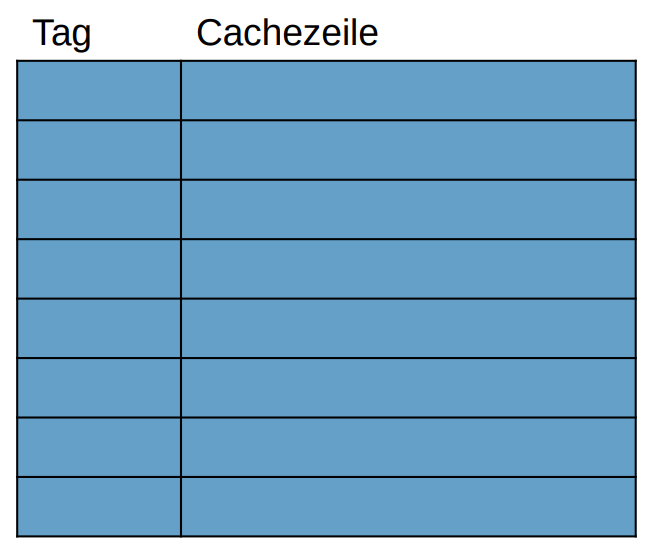
\includegraphics[width=\linewidth]{w05_vollassoz_rep.png}
    \end{column}
  \end{columns}
\end{frame}

\begin{frame}[c]{Cachearten: Mengenassoziativer Cache}{}
  \begin{columns}[c]
    \begin{column}{0.5\textwidth}
      \begin{itemize}
        \item Ein Datum kann auf eine Teilmenge der Cachezeilen gemapped werden (Index) 
        \item Bei Zugriff müssen die Tags innerhalb der Menge angeschaut werden $\rightarrow$ relativ effizienter Zugriff 
        \item Verdrängung eines Datums nur, wenn die Menge voll ist $\rightarrow$  weniger Verdrängungen, und wenn verdrängt wird, dann ein Datum, dass länger nicht gebraucht wurde
        \item Kombination aus Direct-Mapped und Vollassoziativ
      \end{itemize}
    \end{column}
    \begin{column}{0.5\textwidth}
      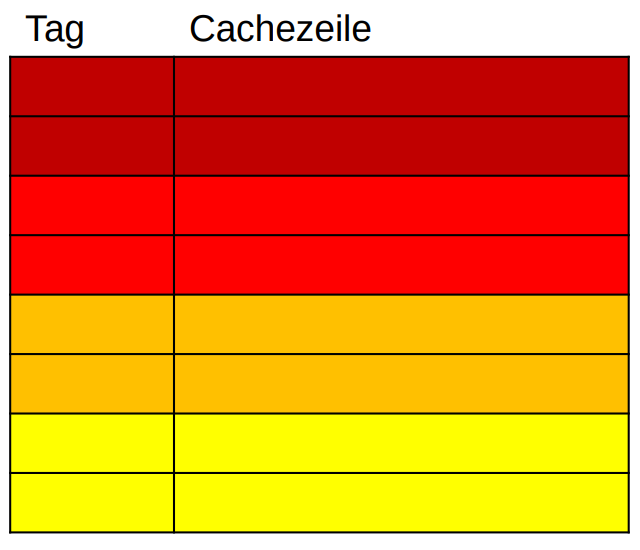
\includegraphics[width=\linewidth]{w05_mengenassoz_rep.png}
    \end{column}
  \end{columns}
\end{frame}

\begin{frame}[c]{Übersicht: Berechnung der Bits für Tag, Index, Offset}{}
  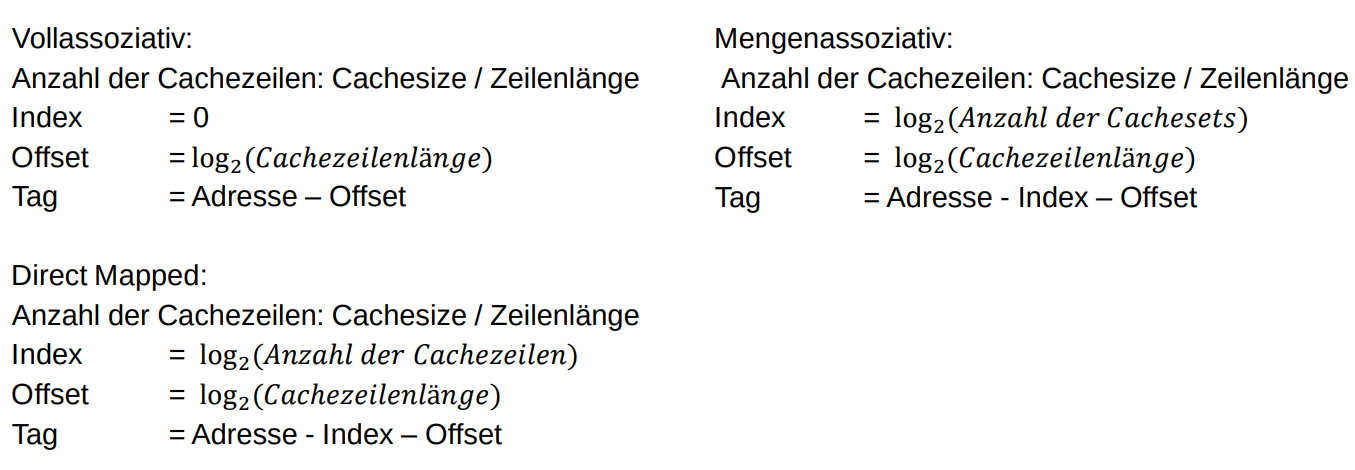
\includegraphics[width=\linewidth]{w05_berechnung_der_bits_rep.png}
\end{frame}

\begin{frame}[c]{Berechnungsbeispiel: Cache-Bits}{}
  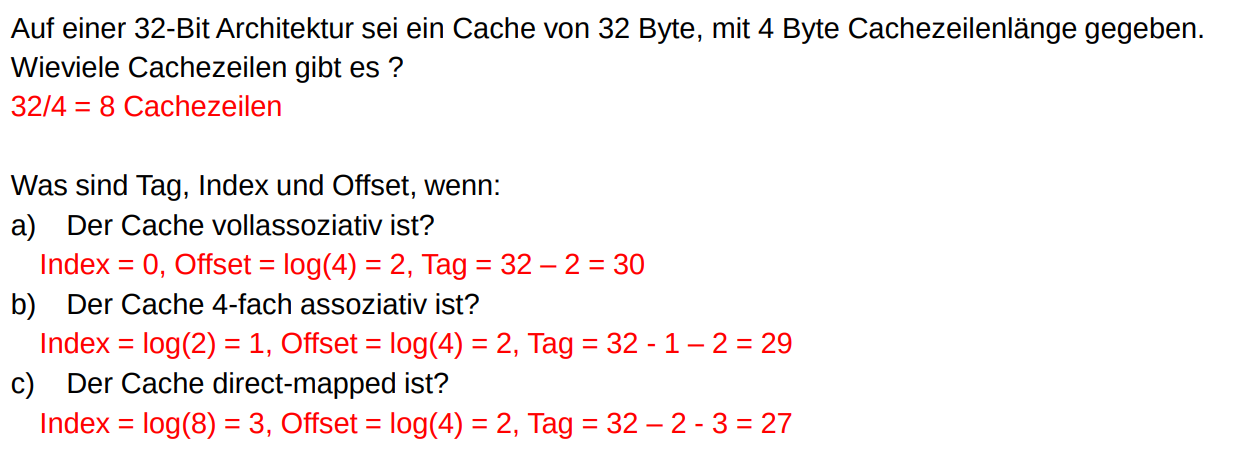
\includegraphics[width=\linewidth]{w05_berechnungsbeispiel1_rep.png}
\end{frame}

\begin{frame}[c]{Berechnungsbeispiel: Cache-Mapping}{}
  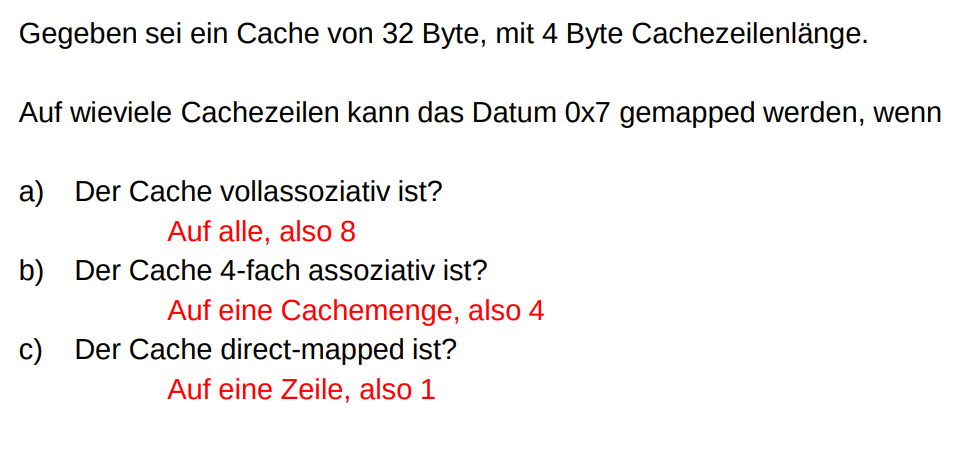
\includegraphics[width=0.8\linewidth]{w05_berechungsbesipiel_mapping_rep.png}
\end{frame}

\begin{frame}[c]{Klassifikation von Misses}{}
  \begin{itemize}
      \item Cold Miss:
      \begin{itemize}
          \item Die Daten an dieser Adresse werden zum ersten Mal in den Cache geladen.
      \end{itemize}
      \item Conflict Miss:
      \begin{itemize}
          \item Die Daten an dieser Adresse waren bereits im Cache, wurden aber verdrängt, obwohl noch Platz im Cache war.
      \end{itemize}
      \item Capacity Miss:
      \begin{itemize}
          \item Die Daten an dieser Adresse waren bereits im Cache, wurden aber verdrängt. Dies wäre selbst bei einem vollassoziativen Cache geschehen.
      \end{itemize}
  \end{itemize}
\end{frame}

\begin{frame}[c]{Graph: Klassifikation von Misses}{}
  \resizebox{\textwidth}{!}{
      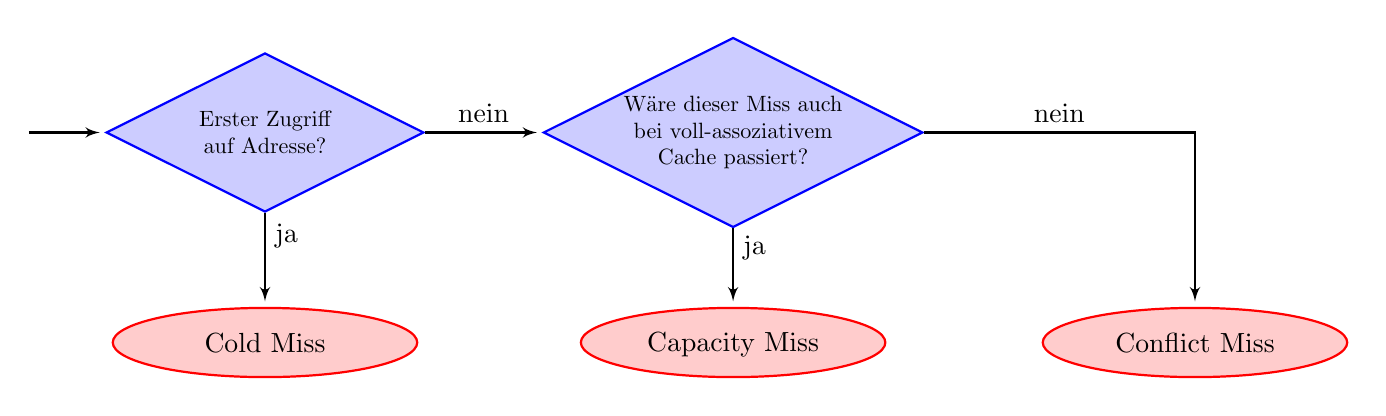
\begin{tikzpicture}
          [auto,
          ampersand replacement=\&,
          decision/.style={diamond, draw=blue, thick, fill=blue!20, text width=35mm, align=center, inner sep=1pt, scale=0.8, aspect=2},
          line/.style={draw, thick, -latex',shorten >=2pt},
          cloud/.style={draw=red, thick, ellipse,fill=red!20,
              minimum height=2.5em, text width=25mm, align=center, text depth=0pt}]
          
          \matrix [column sep=15mm,row sep=10mm]
          {
              \node [decision] (iscoldmiss) {Erster Zugriff auf Adresse?};
              \& \node [decision] (iscapmiss) {Wäre dieser Miss auch bei voll-assoziativem Cache passiert?}; \&\\
              \node [cloud] (coldmiss) {Cold Miss};
              \& \node [cloud] (capacitymiss) {Capacity Miss};
              \& \node [cloud] (conflictmiss) {Conflict Miss};\\
          };
          \begin{scope}[every path/.style=line]
              \path (iscoldmiss) + (left:30mm) -- (iscoldmiss);
              \path (iscoldmiss) -- node [near start] {ja} (coldmiss);
              \path (iscoldmiss) -- node [midway] {nein} (iscapmiss);
              \path (iscapmiss)  -- node [near start] {ja} (capacitymiss);
              \path (iscapmiss)  -| node [near start] {nein} (conflictmiss);
          \end{scope}
  \end{tikzpicture}}
\end{frame}


\begin{frame}{Ersetzungsstrategien}
  \begin{itemize}
      \item LRU (Least Recently Used)
      \begin{itemize}
        \item Löscht die Zeile, auf die am längsten nicht zugegriffen wurde
        \item Gute Leistung bei vielen sequenziellen Zugriffen
        \item Schlecht bei zufälligen oder verstreuten Zugriffen
      \end{itemize}
      \item LFU (Least Frequently Used)
      \begin{itemize}
        \item Löscht die Zeile, auf die am seltensten zugegriffen wurde
        \item Gute Leistung bei repetitiven Zugriffsmustern
        \item Schlecht bei ungleichmäßigen Zugriffsmustern
        \item Erhöhter Overhead durch Zählerverwaltung
      \end{itemize}
      \item FIFO (First in, first out)
      \begin{itemize}
        \item Löscht die zuerst hinzugefügte Zeile
      \end{itemize}
  \end{itemize}
\end{frame}

\begin{frame}[c]{}{}
  \begin{center}
    \LARGE Fragen?
  \end{center}
  \vspace{0.5cm}
  \begin{center}
    \LARGE Bis zum nächsten Mal ;) \\
  \end{center}
  \vspace{1.0cm}
  \begin{center}
    \small Folien inspiriert von Niklas Ladurner \& ZÜ
  \end{center}
\end{frame}

\end{document}